\subsection{Anterior à modificação}

A região escolhida para o cenário 1 foi a interligação entre a subestação de Bouca e Zezere, na região central de Portugal como pode ser visto na Figura \ref{fig:caso1}. A mudança no cenário atual é a retirada de uma das duas linha que interligam o barramento da subestação de Bouca com o barramento de 145 kV de Zezere, o qual pode ser vista na Figura \ref{fig:caso1After}.

\vspace{3.3mm}

\begin{figure}[H]
	\centering
	\captionsetup{width=1\textwidth, font=footnotesize, textfont=bf}	
	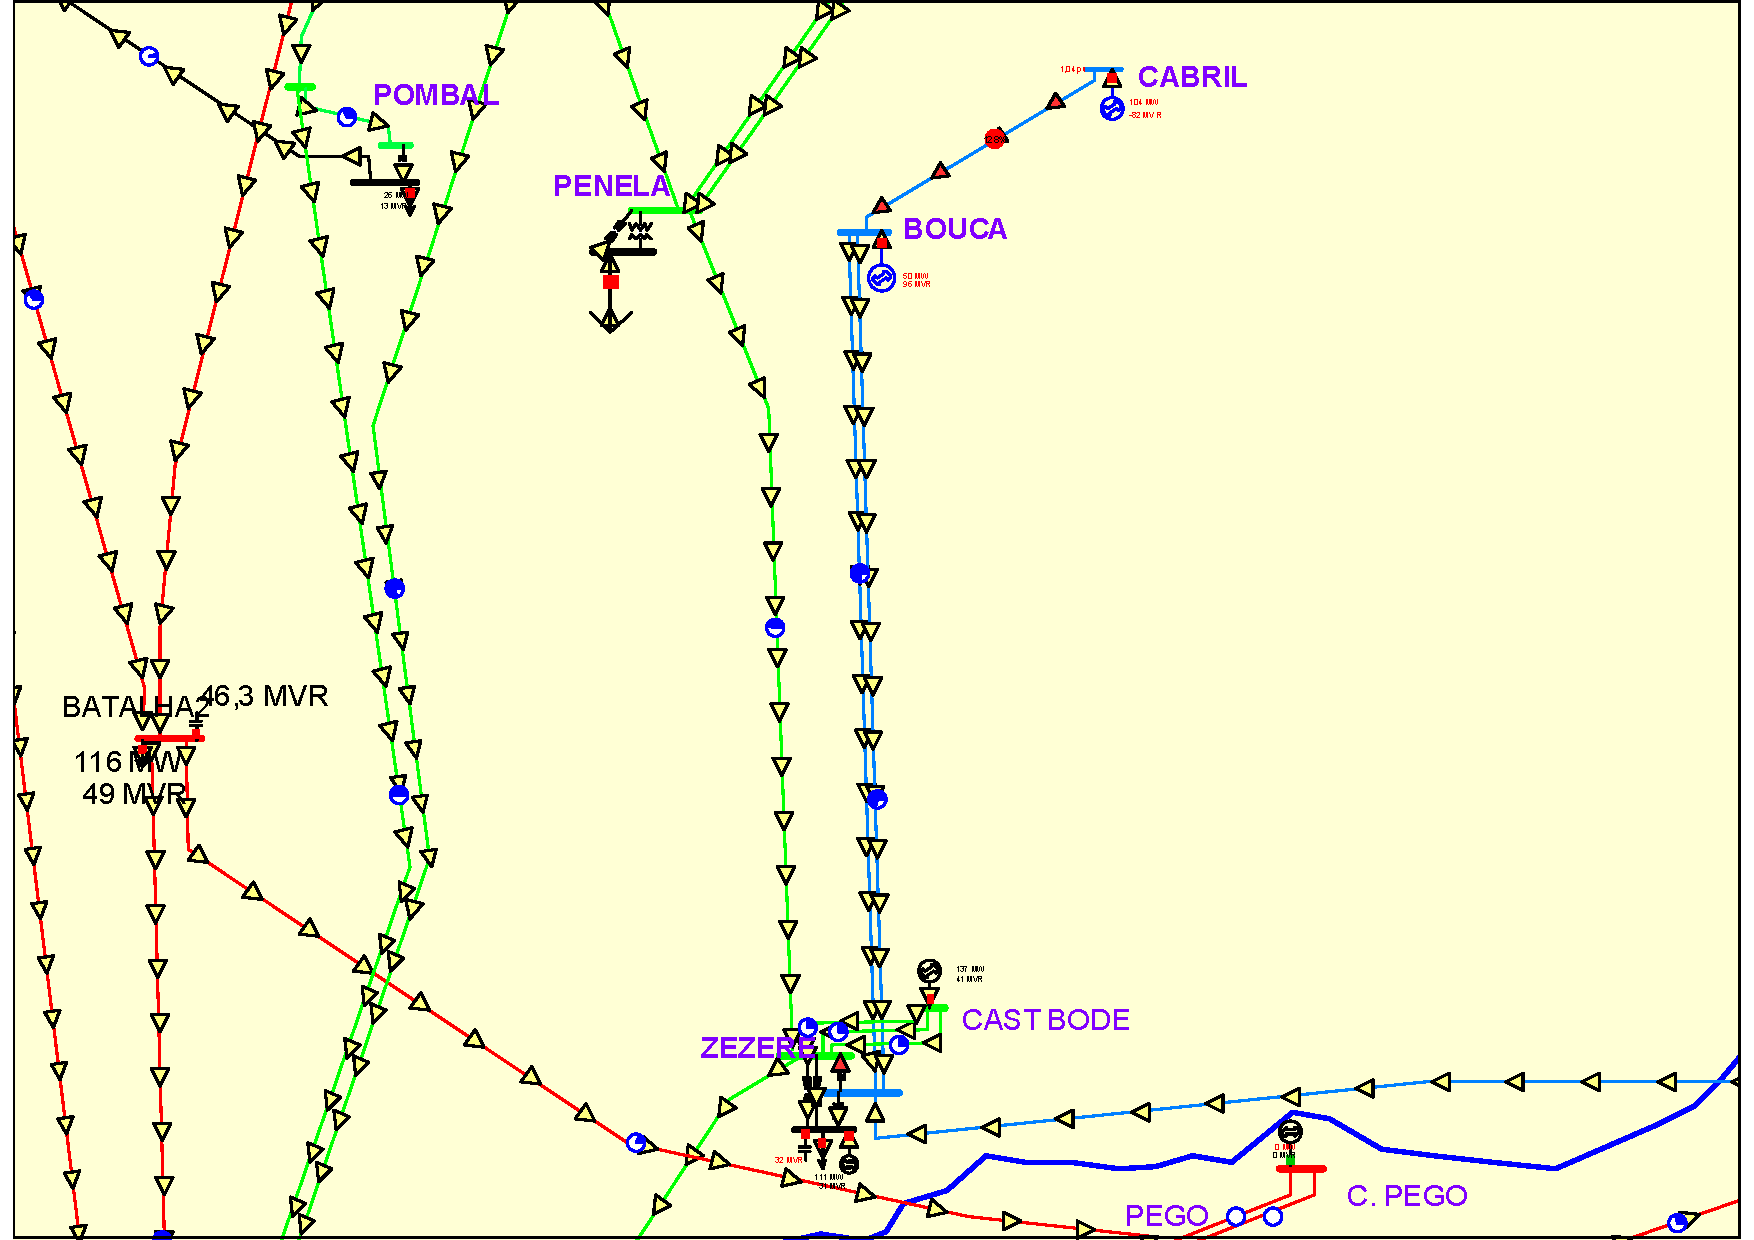
\includegraphics[width=1\linewidth]{img/caso1.pdf}
	\caption{Cenário 1, anterior à modificação}
	\vspace{-3.5mm}
	\caption*{Fonte: Caso Simulado no \textit{PowerWorld\textsuperscript{\textregistered} Simulator}}
	\label{fig:caso1}
\end{figure}

A subestação de Bouca se interliga apenas com o barramento de 145 kV de Zezere e com o barramento de Cabril, o qual possui uma unidade geradora de 104 MW. Existe apenas uma linha de Bouca a Zezere o qual apresenta uma sobrecarga 128\% no transito de potência no sentido Cabril Bouca. A interligação entre bouca e Zezere é feita por duas linhas que apresentam respectivamente  72,5\% e 72,6\% de carregamento.

A subestação de Zezere possui 3 barramentos; o primeiro de 145 kV que interligam a Bouca e Falaguei, o segundo que 230 kV que interligam Santarem, Penela e Cast Bode. O terceiro barramento de 63 kV é onde está conectado uma carga de 111M e um gerador de 22,1 MW. Os dados globais do sistema antes das alterações propostas estão dispostas na tabela \ref{tab:DadosGeraisIniciais}. Já os dados locais relativos as barras próximas a modificação proposta, estão dispostos na Tabela \ref{tab:DadosLocaisIniciais}.

\begin{table}[H]
	\centering
	\captionsetup{width=0.6\textwidth, font=footnotesize, textfont=bf}
	\begin{tabular}{lcc}
		\multicolumn{3}{c}{\cellcolor[HTML]{333333}{\color[HTML]{FFFFFF} Carregamento das Linhas}} \\
		\multicolumn{2}{c}{\textbf{Linhas}}                       & \textbf{Carregamento (\%)}     \\
		Cabril                & \multicolumn{1}{l}{Bouca}         & 128,5                          \\
		Bouca                 & \multicolumn{1}{l}{Zezere}        & 73,4                           \\
		Falaguei              & \multicolumn{1}{l}{Zezere}        & 52,6                           \\
		Panela                & \multicolumn{1}{l}{Zezere}        & 47,1                           \\
		Zezere                & \multicolumn{1}{l}{Santarem}      & 81,5                           \\
		Cast Bode             & \multicolumn{1}{l}{Zezere}        & 25                             \\
		\multicolumn{3}{c}{\cellcolor[HTML]{333333}{\color[HTML]{FFFFFF} Tensão nas Barras}}       \\
		\textbf{Barra}        & \textbf{Módulo}                   & \textbf{Ângulo}                \\
		Cabril                & 1,04                              & 30,889                         \\
		Bouca                 & 1,05                              & 29,566                         \\
		Zezere                & 1,0399                            & 22,006                         \\
		Falaguei              & 1,03                              & 30,919                         \\
		Panela                & 1,0473                            & 26,098                         \\
		Santarem              & 1,0269                            & 14,32                          \\
		Cast Bode             & 1,04                              & 22,019                         \\
		\multicolumn{3}{c}{\cellcolor[HTML]{333333}{\color[HTML]{FFFFFF} Geradores}}               \\
		\textbf{Gerador}      & \textbf{MW}                       & \textbf{Mvar}                  \\
		Cabril                & 104,2                             & -82,29                         \\
		Bouca                 & 49,6                              & 96,14                          \\
		Zezere                & 22,1                              & -23,24                         \\
		Cast Bode             & 137,2                             & 41,46                          \\
		Falaguei              & 148                               & 65,76                          \\   
	\end{tabular}
	\caption{Dados Locais Antes das Modificações - Caso 1}
  	\vspace{-3.5mm}
	\caption*{Fonte: Autoria Própria}
  	\label{tab:DadosLocaisIniciais}
\end{table}

\begin{table}[H]
	\centering
	\captionsetup{width=0.4\textwidth, font=footnotesize, textfont=bf}
	\begin{tabular}{|
			>{\columncolor[HTML]{333333}}l |c|c|l}
		\cline{1-3}
		{\color[HTML]{FFFFFF} }        & \cellcolor[HTML]{333333}{\color[HTML]{FFFFFF} MW} & \cellcolor[HTML]{333333}{\color[HTML]{FFFFFF} MVAr} &  \\ \cline{1-3}
		{\color[HTML]{FFFFFF} Perdas}  & 229,50                                            & -376,75  &  \\ \cline{1-3}
		{\color[HTML]{FFFFFF} Geração} & 6794,0                                             & -306,1  &  \\ \cline{1-3}
		{\color[HTML]{FFFFFF} Cargas}  & 6564,5                                            & 1814,2 &  \\ \cline{1-3}
	\end{tabular}
	\caption{Dados globais iniciais}
	\vspace{-3.5mm}
	\caption*{Fonte: Autoria Própria}
	\label{tab:DadosGeraisIniciais}
\end{table}


\subsection{Análise do impacto da modificação}

\begin{figure}[H]
	\centering
	\captionsetup{width=1\textwidth, font=footnotesize, textfont=bf}	
	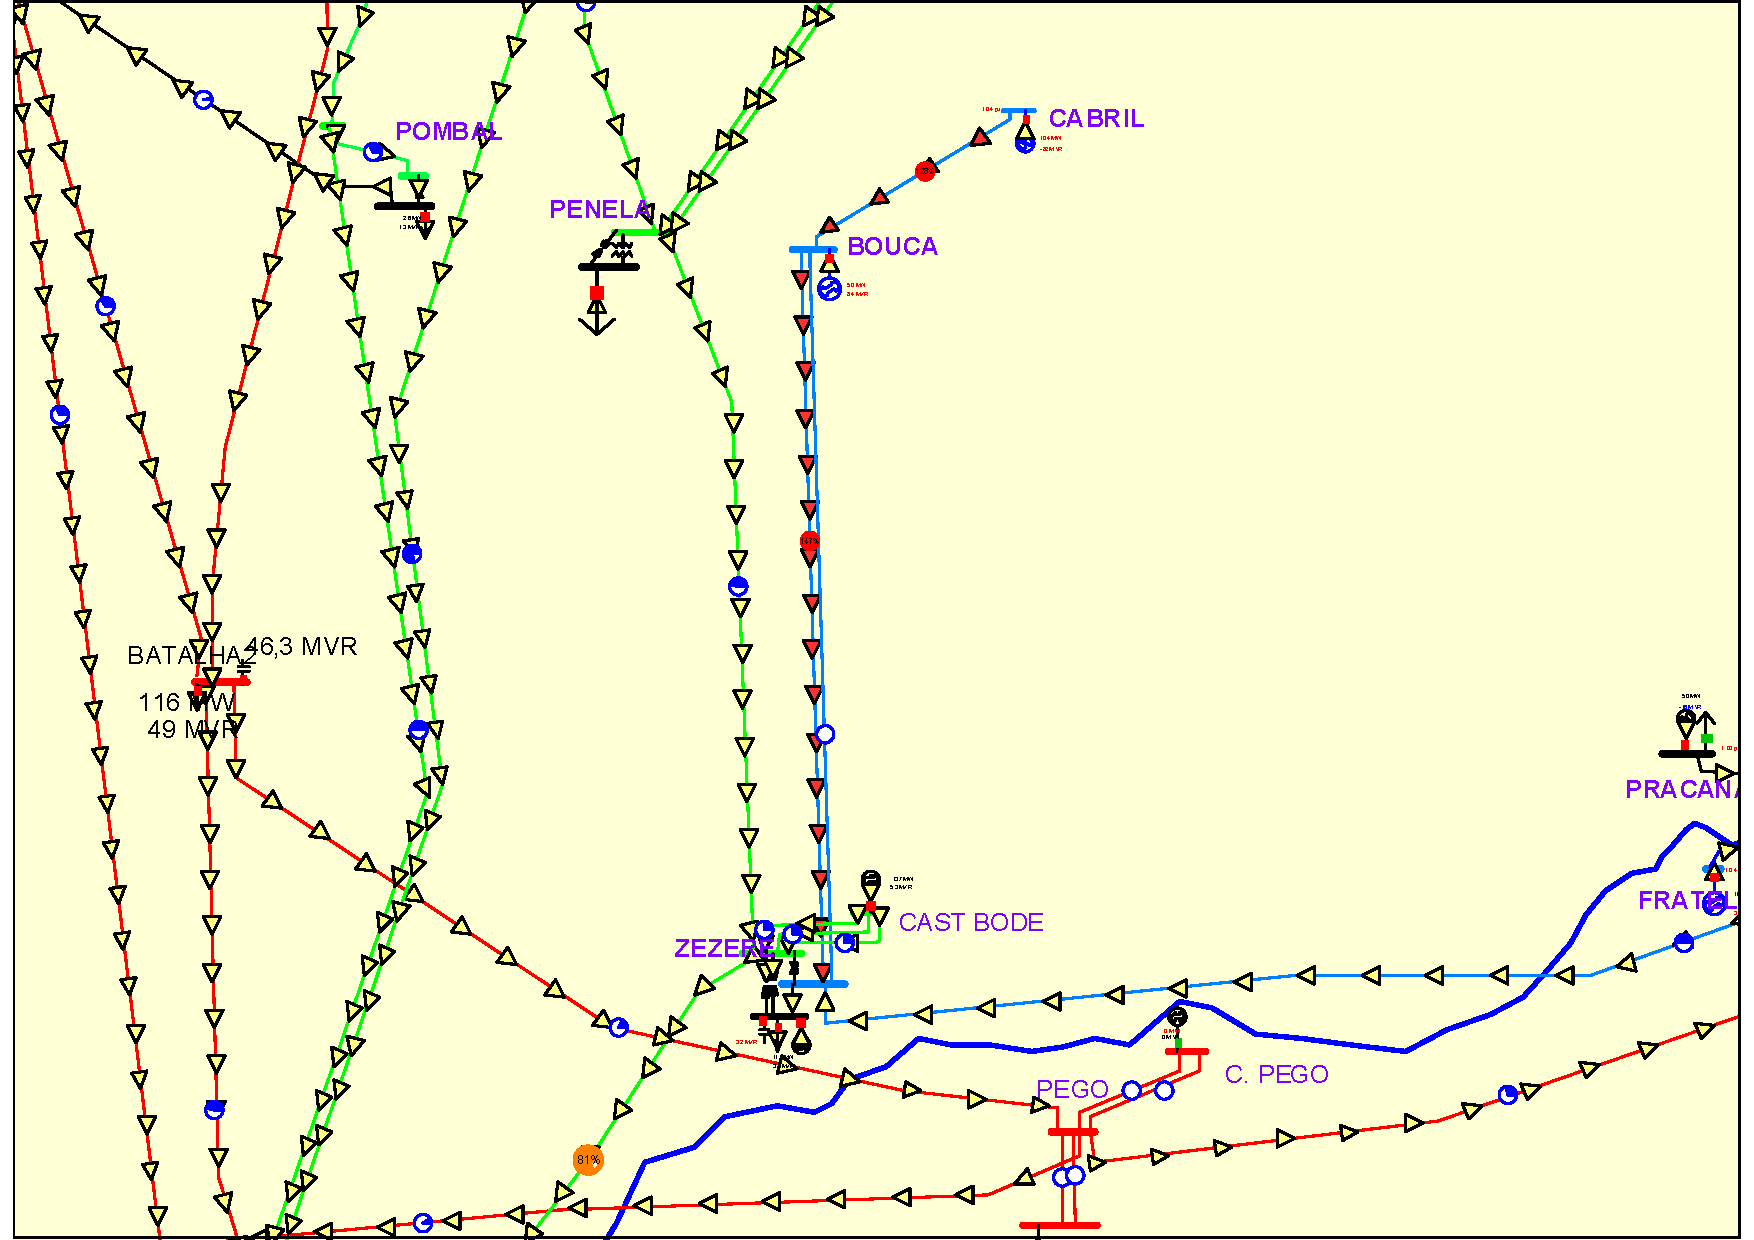
\includegraphics[width=1\linewidth]{img/caso1After.pdf}
	\caption{Cenário 1, após à modificação}
	\vspace{-3.5mm}
	\caption*{Fonte: Caso Simulado no \textit{PowerWorld\textsuperscript{\textregistered} Simulator}}
	\label{fig:caso1After}
\end{figure}

\begin{table}[H]
	\centering
	\captionsetup{width=0.6\textwidth, font=footnotesize, textfont=bf}
	\begin{tabular}{lcc}
		\multicolumn{3}{c}{\cellcolor[HTML]{333333}{\color[HTML]{FFFFFF} Carregamento das Linhas}}                              \\
		\multicolumn{2}{c}{{\color[HTML]{333333} \textbf{Linhas}}}          & {\color[HTML]{333333} \textbf{Carregamento (\%)}} \\
		Cabril                               & \multicolumn{1}{l}{Bouca}    & 128,5                                             \\
		Bouca                                & \multicolumn{1}{l}{Zezere}   & 147                                               \\
		Falaguei                             & \multicolumn{1}{l}{Zezere}   & 52                                                \\
		Panela                               & \multicolumn{1}{l}{Zezere}   & 47,2                                              \\
		Zezere                               & \multicolumn{1}{l}{Santarem} & 81,4                                              \\
		Cast Bode                            & \multicolumn{1}{l}{Zezere}   & 25,7                                              \\
		\multicolumn{3}{c}{\cellcolor[HTML]{333333}{\color[HTML]{FFFFFF} Tensão nas Barras}}                                    \\
		\multicolumn{1}{l}{\textbf{Barra}}   & \textbf{Módulo}              & \textbf{Ângulo}                                   \\
		Cabril                               & 1,04                         & 33,743                                            \\
		Bouca                                & 1,05                         & 32,42                                             \\
		Zezere                               & 1,0399                       & 21,96                                             \\
		Falaguei                             & 1,03                         & 30,855                                            \\
		Panela                               & 1,0473                       & 26,058                                            \\
		Santarem                             & 1,0269                       & 14,283                                            \\
		Cast Bode                            & 1,04                         & 21,973                                            \\
		\multicolumn{3}{c}{\cellcolor[HTML]{333333}{\color[HTML]{FFFFFF} Geradores}}                                            \\
		\multicolumn{1}{l}{\textbf{Gerador}} & \textbf{MW}                  & \textbf{Mvar}                                     \\
		Cabril                               & 104,2                        & -82,29                                            \\
		Bouca                                & 49,6                         & 83,9                                              \\
		Zezere                               & 22,1                         & -19,07                                            \\
		Cast Bode                            & 137,2                        & 52,65                                             \\
		Falaguei                             & 148                          & 72,05                                             \\                                  
	\end{tabular}
	\caption{Dados Locais Após a Modificação - Caso 1}
	\vspace{-3.5mm}
	\caption*{Fonte: Autoria Própria}
	\label{tab:DadosLocaisFinaisCaso1}
\end{table}

\begin{table}[H]
	\centering
	\captionsetup{width=0.4\textwidth, font=footnotesize, textfont=bf}
	\begin{tabular}{
			>{\columncolor[HTML]{333333}}l ll}
		{\color[HTML]{FFFFFF} }        & \cellcolor[HTML]{333333}{\color[HTML]{FFFFFF} MW} & \cellcolor[HTML]{333333}{\color[HTML]{FFFFFF} Mvar} \\
		{\color[HTML]{FFFFFF} Carga}   & 6564,5                                            & 1814,2                                              \\
		{\color[HTML]{FFFFFF} Geração} & 6795,9                                            & -298,3                                              \\
		{\color[HTML]{FFFFFF} Perdas}  & 231,42                                            & -368,86                                            
	\end{tabular}
	\caption{Dados Globais Após a Alteração}
	\vspace{-3.5mm}
	\caption*{Fonte: Autoria Própria}
	\label{tab:DadosGeraisAposAlteracaoCaso1}
\end{table}

\subsubsection{Análise global}

\begin{figure}[H]
	\centering
	\captionsetup{width=\textwidth, font=footnotesize, textfont=bf}	
	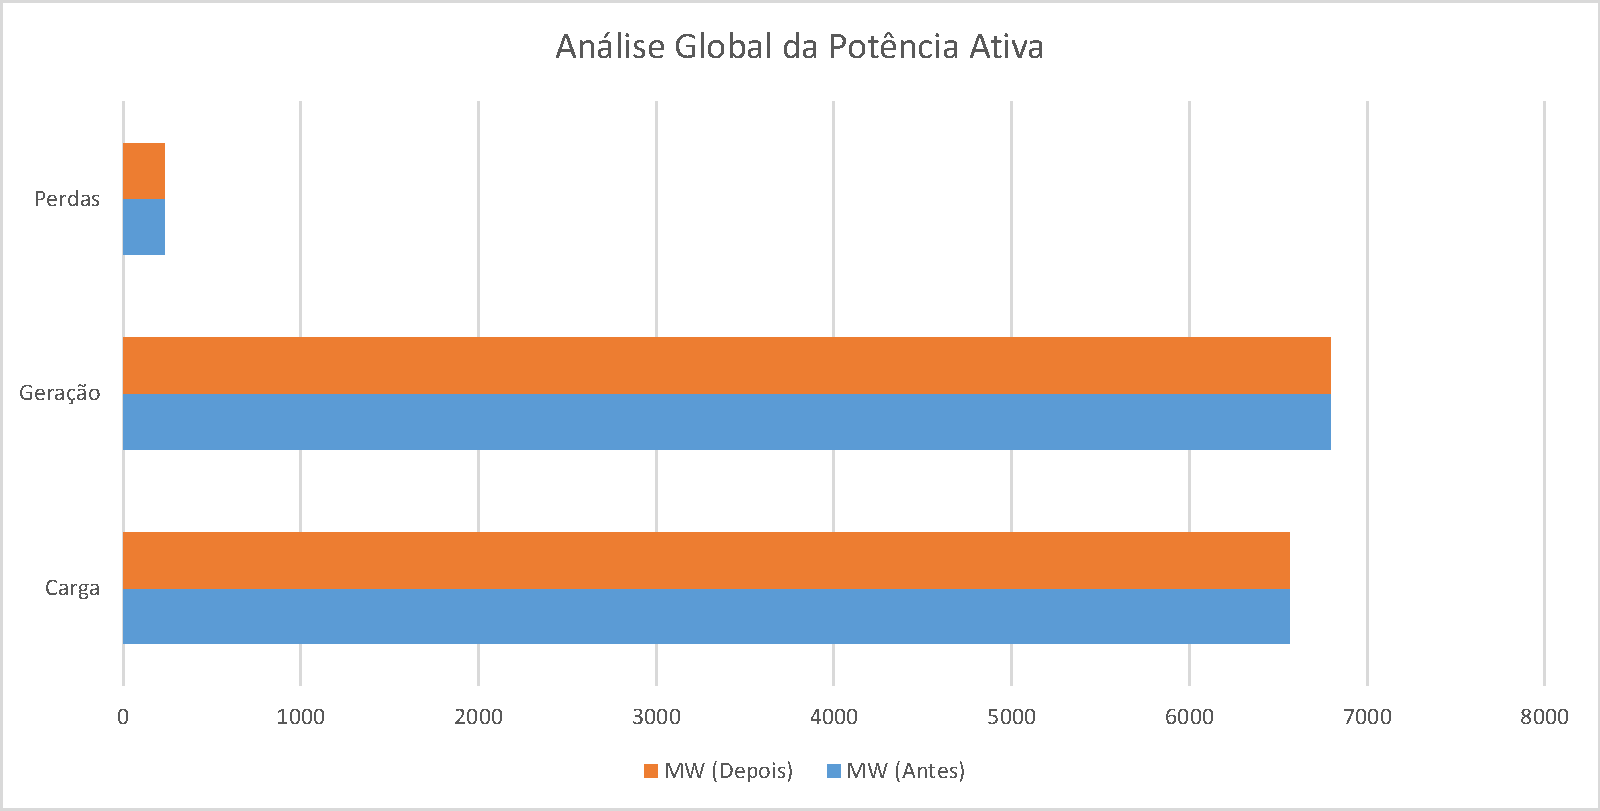
\includegraphics[width=\linewidth]{img/global_MW_caso1.pdf}
	\caption{Análise ativa global antes e após o cenário 1}
	\vspace{-3.5mm}
	\caption*{Fonte: autoria própria}
	\label{fig:global_MW_caso1}
\end{figure}

\begin{figure}[H]
	\centering
	\captionsetup{width=\textwidth, font=footnotesize, textfont=bf}	
	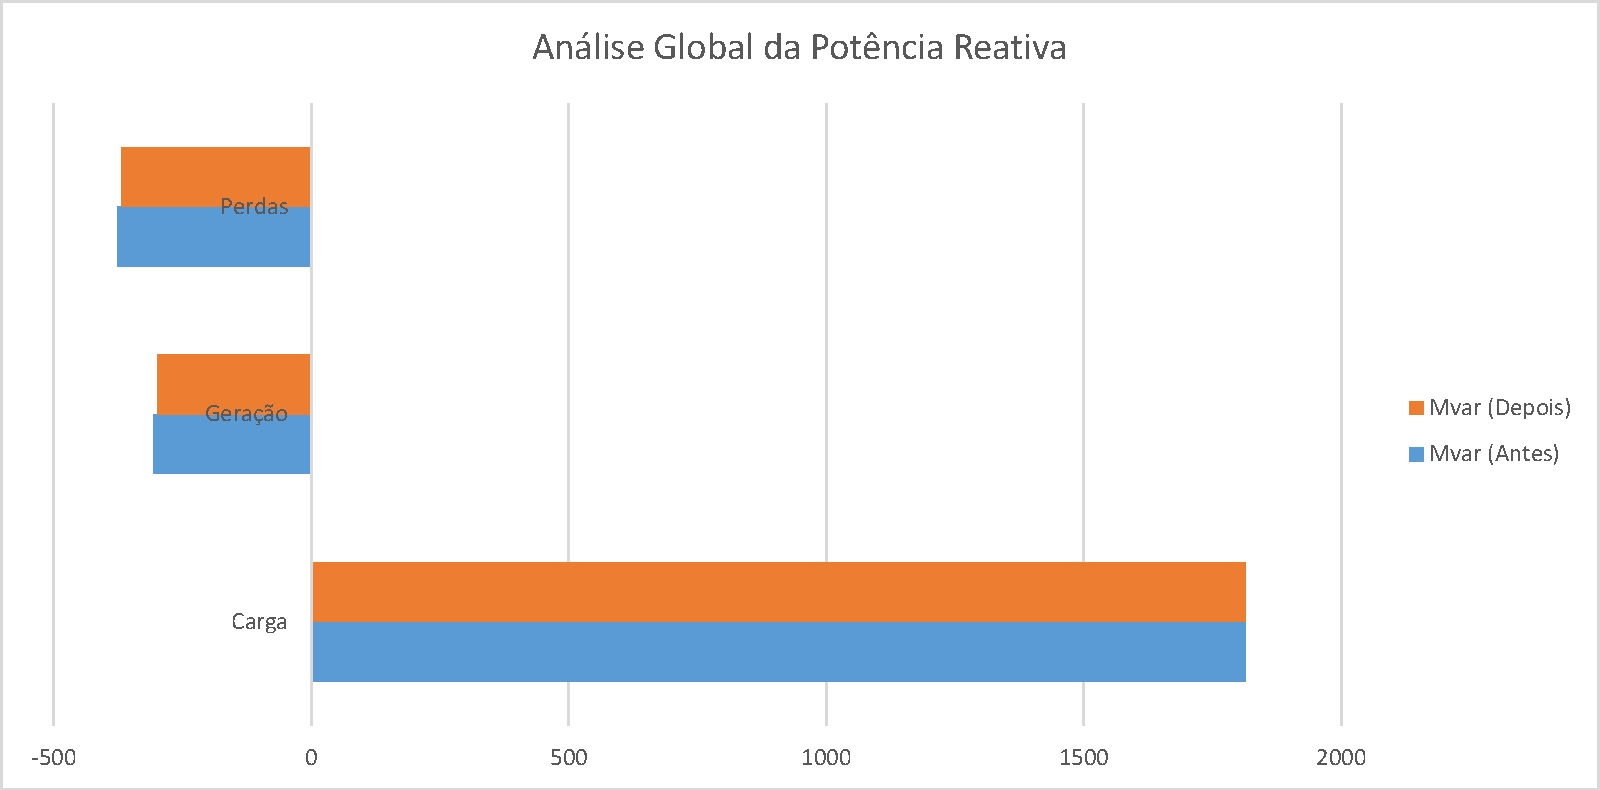
\includegraphics[width=\linewidth]{img/global_MVAr_caso1.pdf}
	\caption{Análise reativa global antes e após o cenário 1}
	\vspace{-3.5mm}
	\caption*{Fonte: autoria própria}
	\label{fig:global_MVAr_caso1}
\end{figure}
\subsubsection{Análise geradores}

\begin{figure}[H]
	\centering
	\captionsetup{width=\textwidth, font=footnotesize, textfont=bf}	
	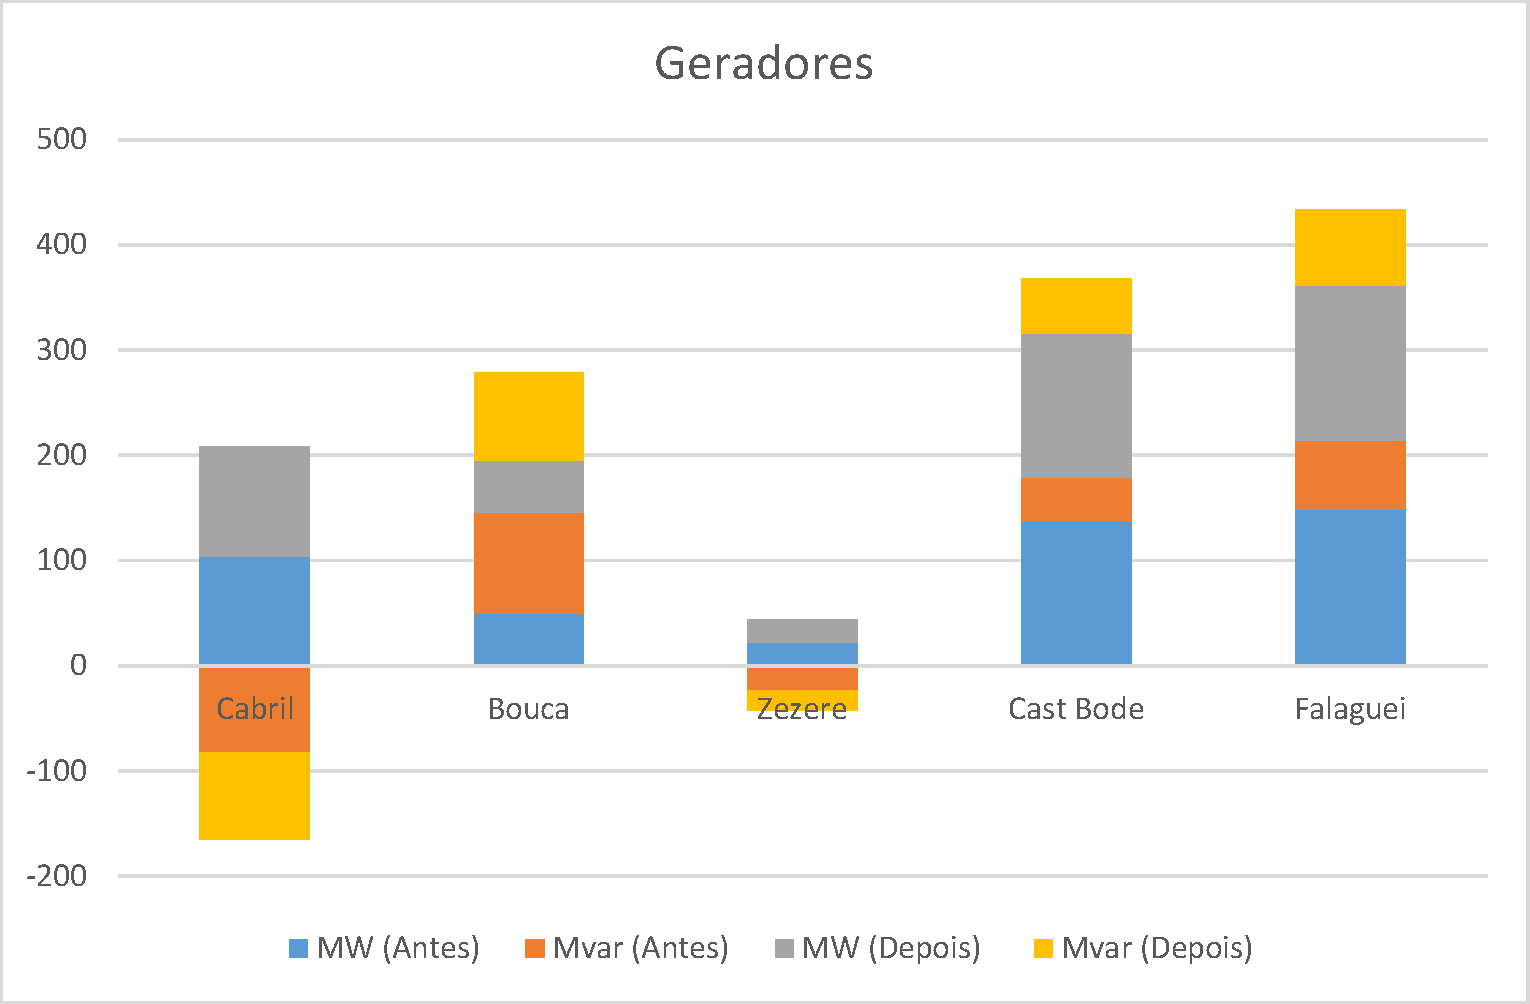
\includegraphics[width=\linewidth]{img/geradores_caso1.pdf}
	\caption{Análise dos geradores antes e após o cenário 1}
	\vspace{-3.5mm}
	\caption*{Fonte: autoria própria}
	\label{fig:geradores_caso1}
\end{figure}


\subsubsection{Análise das linhas}

\begin{figure}[H]
	\centering
	\captionsetup{width=\textwidth, font=footnotesize, textfont=bf}	
	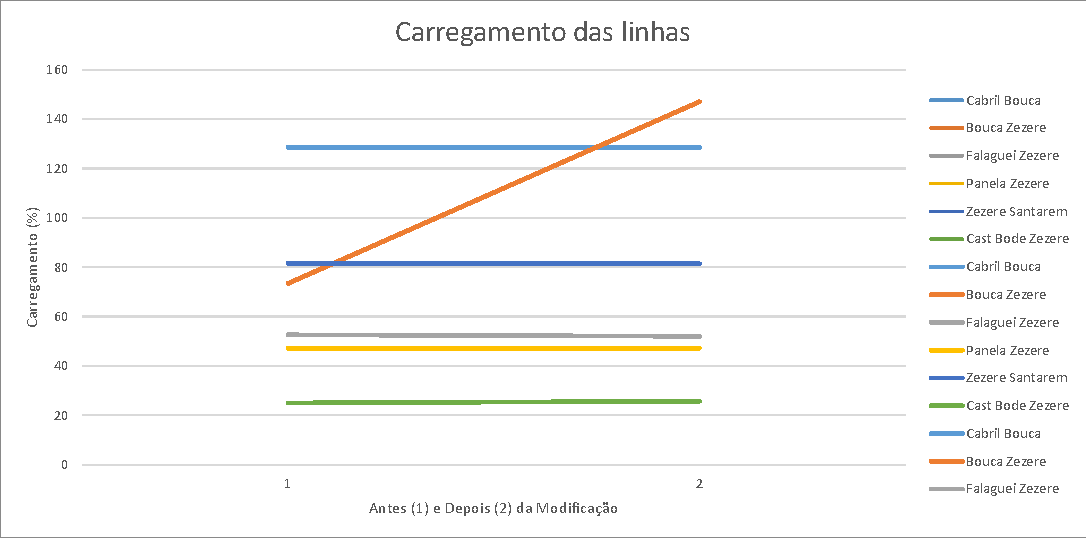
\includegraphics[width=0.9\linewidth]{img/carregamento_linhas_caso1.pdf}
	\caption{Análise do carregamento das linhas antes e após o cenário 1}
	\vspace{-3.5mm}
	\caption*{Fonte: autoria própria}
	\label{fig:carregamento_linhas_caso1}
\end{figure}

	% Mudança do trânsito de potência
	% Sobrecargas
    
\subsubsection{Análise dos Barramentos}

\begin{figure}[H]
	\centering
	\captionsetup{width=\textwidth, font=footnotesize, textfont=bf}	
	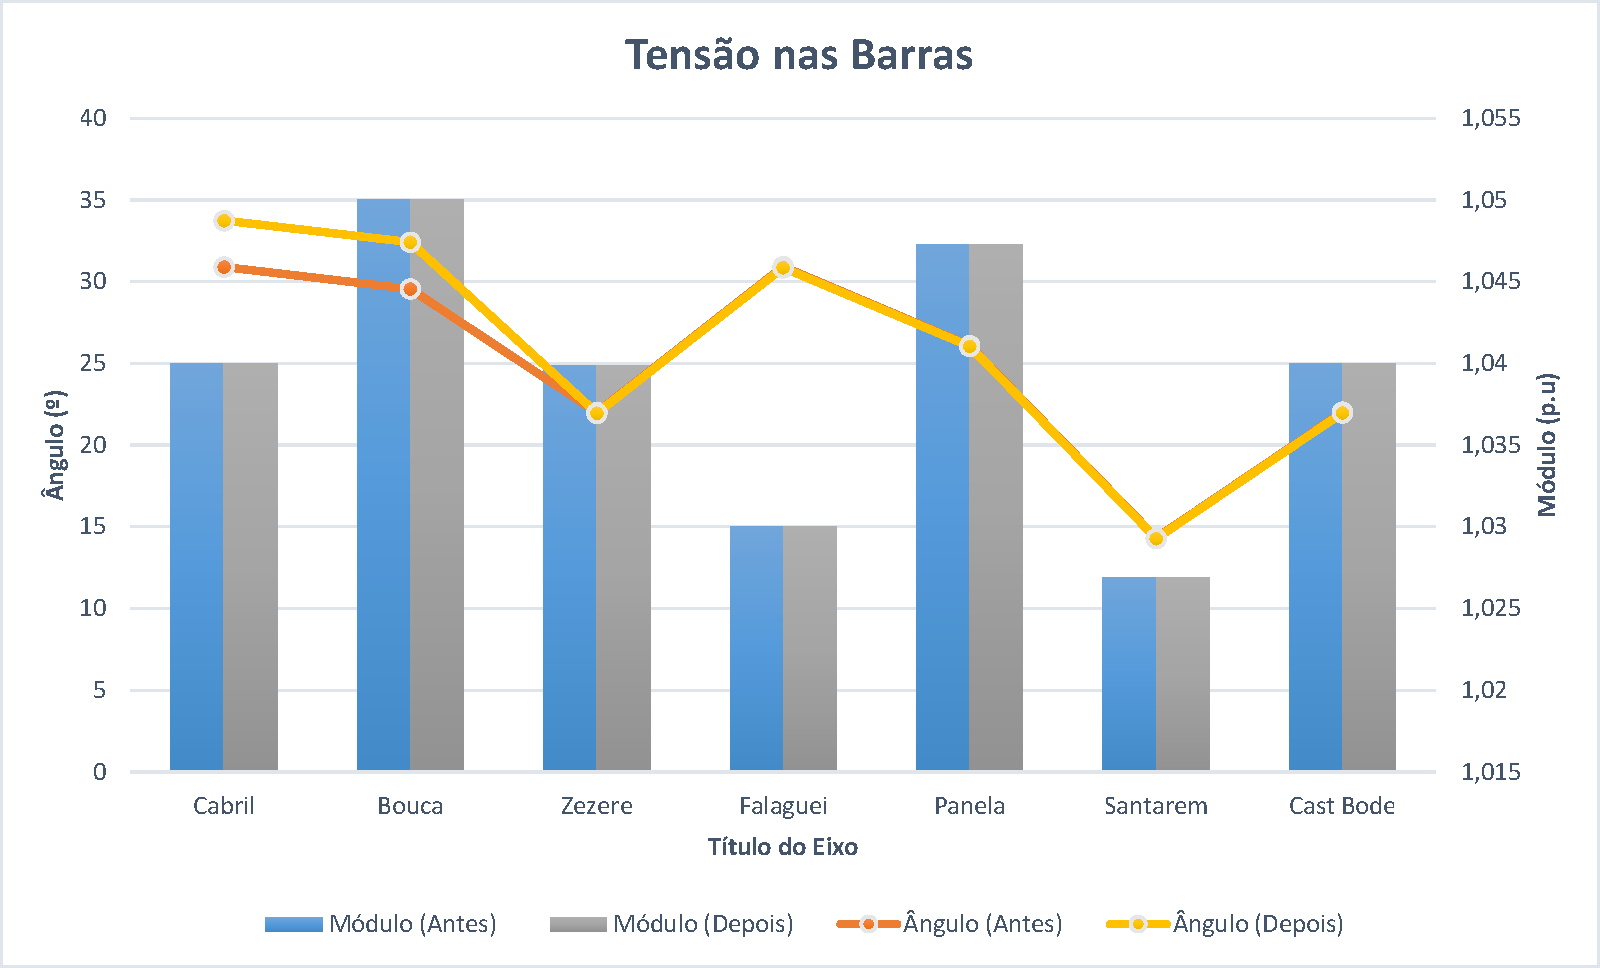
\includegraphics[width=\linewidth]{img/tensoes_barras_caso1.pdf}
	\caption{Análise dos Barramentos Antes e Após o Cenário 1}
	\vspace{-3.5mm}
	\caption*{Fonte: autoria própria}
	\label{fig:tensoes_barras_caso1}
\end{figure}
	% Tensões 
	% Ângulos